\documentclass[conference]{IEEEtran}
\usepackage{cite}
% *** GRAPHICS RELATED PACKAGES ***
%
\ifCLASSINFOpdf
  % \usepackage[pdftex]{graphicx}
  % declare the path(s) where your graphic files are
  % \graphicspath{{../pdf/}{../jpeg/}}
  % and their extensions so you won't have to specify these with
  % every instance of \includegraphics
  % \DeclareGraphicsExtensions{.pdf,.jpeg,.png}
\else
  % or other class option (dvipsone, dvipdf, if not using dvips). graphicx
  % will default to the driver specified in the system graphics.cfg if no
  % driver is specified.
  % \usepackage[dvips]{graphicx}
  % declare the path(s) where your graphic files are
  % \graphicspath{{../eps/}}
  % and their extensions so you won't have to specify these with
  % every instance of \includegraphics
  % \DeclareGraphicsExtensions{.eps}
\fi
% graphicx was written by David Carlisle and Sebastian Rahtz. It is
% required if you want graphics, photos, etc. graphicx.sty is already
% installed on most LaTeX systems. The latest version and documentation
% can be obtained at: 
% http://www.ctan.org/pkg/graphicx
% Another good source of documentation is "Using Imported Graphics in
% LaTeX2e" by Keith Reckdahl which can be found at:
% http://www.ctan.org/pkg/epslatex
%
% latex, and pdflatex in dvi mode, support graphics in encapsulated
% postscript (.eps) format. pdflatex in pdf mode supports graphics
% in .pdf, .jpeg, .png and .mps (metapost) formats. Users should ensure
% that all non-photo figures use a vector format (.eps, .pdf, .mps) and
% not a bitmapped formats (.jpeg, .png). The IEEE frowns on bitmapped formats
% which can result in "jaggedy"/blurry rendering of lines and letters as
% well as large increases in file sizes.
%
% You can find documentation about the pdfTeX application at:
% http://www.tug.org/applications/pdftex

% *** MATH PACKAGES ***
%
%\usepackage{amsmath}
% A popular package from the American Mathematical Society that provides
% many useful and powerful commands for dealing with mathematics.
%
% Note that the amsmath package sets \interdisplaylinepenalty to 10000
% thus preventing page breaks from occurring within multiline equations. Use:
%\interdisplaylinepenalty=2500
% after loading amsmath to restore such page breaks as IEEEtran.cls normally
% does. amsmath.sty is already installed on most LaTeX systems. The latest
% version and documentation can be obtained at:
% http://www.ctan.org/pkg/amsmath

% *** SPECIALIZED LIST PACKAGES ***
%
%\usepackage{algorithmic}
% algorithmic.sty was written by Peter Williams and Rogerio Brito.
% This package provides an algorithmic environment fo describing algorithms.
% You can use the algorithmic environment in-text or within a figure
% environment to provide for a floating algorithm. Do NOT use the algorithm
% floating environment provided by algorithm.sty (by the same authors) or
% algorithm2e.sty (by Christophe Fiorio) as the IEEE does not use dedicated
% algorithm float types and packages that provide these will not provide
% correct IEEE style captions. The latest version and documentation of
% algorithmic.sty can be obtained at:
% http://www.ctan.org/pkg/algorithms
% Also of interest may be the (relatively newer and more customizable)
% algorithmicx.sty package by Szasz Janos:
% http://www.ctan.org/pkg/algorithmicx

% *** ALIGNMENT PACKAGES ***
%
%\usepackage{array}
% Frank Mittelbach's and David Carlisle's array.sty patches and improves
% the standard LaTeX2e array and tabular environments to provide better
% appearance and additional user controls. As the default LaTeX2e table
% generation code is lacking to the point of almost being broken with
% respect to the quality of the end results, all users are strongly
% advised to use an enhanced (at the very least that provided by array.sty)
% set of table tools. array.sty is already installed on most systems. The
% latest version and documentation can be obtained at:
% http://www.ctan.org/pkg/array

% *** SUBFIGURE PACKAGES ***
%\ifCLASSOPTIONcompsoc
%  \usepackage[caption=false,font=normalsize,labelfont=sf,textfont=sf]{subfig}
%\else
%  \usepackage[caption=false,font=footnotesize]{subfig}
%\fi
% subfig.sty, written by Steven Douglas Cochran, is the modern replacement
% for subfigure.sty, the latter of which is no longer maintained and is
% incompatible with some LaTeX packages including fixltx2e. However,
% subfig.sty requires and automatically loads Axel Sommerfeldt's caption.sty
% which will override IEEEtran.cls' handling of captions and this will result
% in non-IEEE style figure/table captions. To prevent this problem, be sure
% and invoke subfig.sty's "caption=false" package option (available since
% subfig.sty version 1.3, 2005/06/28) as this is will preserve IEEEtran.cls
% handling of captions.
% Note that the Computer Society format requires a larger sans serif font
% than the serif footnote size font used in traditional IEEE formatting
% and thus the need to invoke different subfig.sty package options depending
% on whether compsoc mode has been enabled.
%
% The latest version and documentation of subfig.sty can be obtained at:
% http://www.ctan.org/pkg/subfig

% *** FLOAT PACKAGES ***
%
%\usepackage{fixltx2e}
% fixltx2e, the successor to the earlier fix2col.sty, was written by
% Frank Mittelbach and David Carlisle. This package corrects a few problems
% in the LaTeX2e kernel, the most notable of which is that in current
% LaTeX2e releases, the ordering of single and double column floats is not
% guaranteed to be preserved. Thus, an unpatched LaTeX2e can allow a
% single column figure to be placed prior to an earlier double column
% figure.
% Be aware that LaTeX2e kernels dated 2015 and later have fixltx2e.sty's
% corrections already built into the system in which case a warning will
% be issued if an attempt is made to load fixltx2e.sty as it is no longer
% needed.
% The latest version and documentation can be found at:
% http://www.ctan.org/pkg/fixltx2e

%\usepackage{stfloats}
% stfloats.sty was written by Sigitas Tolusis. This package gives LaTeX2e
% the ability to do double column floats at the bottom of the page as well
% as the top. (e.g., "\begin{figure*}[!b]" is not normally possible in
% LaTeX2e). It also provides a command:
%\fnbelowfloat
% to enable the placement of footnotes below bottom floats (the standard
% LaTeX2e kernel puts them above bottom floats). This is an invasive package
% which rewrites many portions of the LaTeX2e float routines. It may not work
% with other packages that modify the LaTeX2e float routines. The latest
% version and documentation can be obtained at:
% http://www.ctan.org/pkg/stfloats
% Do not use the stfloats baselinefloat ability as the IEEE does not allow
% \baselineskip to stretch. Authors submitting work to the IEEE should note
% that the IEEE rarely uses double column equations and that authors should try
% to avoid such use. Do not be tempted to use the cuted.sty or midfloat.sty
% packages (also by Sigitas Tolusis) as the IEEE does not format its papers in
% such ways.
% Do not attempt to use stfloats with fixltx2e as they are incompatible.
% Instead, use Morten Hogholm'a dblfloatfix which combines the features
% of both fixltx2e and stfloats:
%
% \usepackage{dblfloatfix}
% The latest version can be found at:
% http://www.ctan.org/pkg/dblfloatfix

% *** PDF, URL AND HYPERLINK PACKAGES ***
%
%\usepackage{url}
% url.sty was written by Donald Arseneau. It provides better support for
% handling and breaking URLs. url.sty is already installed on most LaTeX
% systems. The latest version and documentation can be obtained at:
% http://www.ctan.org/pkg/url
% Basically, \url{my_url_here}.
\usepackage{graphicx}

\begin{document}

\title{Distributed Tic Tac Toe:\\ Peer-to-Peer Team-Based Gaming System}

\author{Panagiotis Antoniou, Emily Band, Paulius Dilkas, Dafin Kozarev, Joshua Styles}
\maketitle

\begin{abstract}
This article describes a Distributed Multiplayer Tic Tac Toe software game written in Java using the RMI API. While previous implementations attempting to serve a similar purpose exist, none of them boast good design or efficiency and neither of them deliver the same functionality. The developed piece of software allows clients to play locally or globally a game of the classic tic tac toe - but with a twist. Players are separated into teams and decide on what the next move should be by voting. The implementation is derived from a design that follows the distributed applications guidelines and is prepared to handle corner cases such as client disconnects for example.
\end{abstract}

\section{Introduction}
Coding is the main occupation of many people nowadays, and it is a
past-time for many too. Most beginners get their first steps in writing code
following the local single-threaded model. Often, it can be difficult for
new programmers, or even those with more experience, to abstract the key
knowledge they have obtained using this model and then apply it in a different way.

Distributed software requires a new look on the system – the number of devices
has gone up and with it so have the number of processes, concerns and complexities.
Some concepts have now changed and need to be dealt with differently; One such
example if this would be mutual exclusion. We believe programs that serve as examples and
focus on simple local tasks turned into distributed ones can help many people
trying to make this step with a hands-on experience of what they are preparing
for. Seeing theory in practice is a proven technique and there is evidence for
this in every university course that features practical work. This is especially
true where games are concerned, proving to be an effective means of communicating 
programming methods and techniques in an engaging way
\cite{Kiniry:2011:VG:1984674.1984681}. For this reason, the team has decided to
take a simple, well known game and develop it into a distributed system; Tic Tac
Toe played as a peer-to-peer, team-based gaming system where the players are
organised into teams and required to vote on moves for their team.

By refraining from introducing additional complexity as part of the goal of the project, and 
allowing the users to see the distributed nature of the software being demonstrated via a simple game, the focus is shifted towards the implications of the distributive aspects of the system and 
the way they are handled. The finished product can serve to entertain the end users, as well as increase their curiosity and insight about computers and distributed systems. Using Tic Tac Toe as a foundation to demonstrate a distributed system benefits from both the simplicity and familiarity of the game itself, meaning no complex rulesets or in-depth mechanisms need be explained to the users, allowing the distributed nature to be a novel way of experiencing a widely known game.

% An example of a floating figure using the graphicx package.
% Note that \label must occur AFTER (or within) \caption.
% For figures, \caption should occur after the \includegraphics.
% Note that IEEEtran v1.7 and later has special internal code that
% is designed to preserve the operation of \label within \caption
% even when the captionsoff option is in effect. However, because
% of issues like this, it may be the safest practice to put all your
% \label just after \caption rather than within \caption{}.
%
% Reminder: the "draftcls" or "draftclsnofoot", not "draft", class
% option should be used if it is desired that the figures are to be
% displayed while in draft mode.
%
%\begin{figure}[!t]
%\centering
%\includegraphics[width=2.5in]{myfigure}
% where an .eps filename suffix will be assumed under latex, 
% and a .pdf suffix will be assumed for pdflatex; or what has been declared
% via \DeclareGraphicsExtensions.
%\caption{Simulation results for the network.}
%\label{fig_sim}
%\end{figure}

% Note that the IEEE typically puts floats only at the top, even when this
% results in a large percentage of a column being occupied by floats.

% An example of a double column floating figure using two subfigures.
% (The subfig.sty package must be loaded for this to work.)
% The subfigure \label commands are set within each subfloat command,
% and the \label for the overall figure must come after \caption.
% \hfil is used as a separator to get equal spacing.
% Watch out that the combined width of all the subfigures on a 
% line do not exceed the text width or a line break will occur.
%
%\begin{figure*}[!t]
%\centering
%\subfloat[Case I]{\includegraphics[width=2.5in]{box}%
%\label{fig_first_case}}
%\hfil
%\subfloat[Case II]{\includegraphics[width=2.5in]{box}%
%\label{fig_second_case}}
%\caption{Simulation results for the network.}
%\label{fig_sim}
%\end{figure*}
%
% Note that often IEEE papers with subfigures do not employ subfigure
% captions (using the optional argument to \subfloat[]), but instead will
% reference/describe all of them (a), (b), etc., within the main caption.
% Be aware that for subfig.sty to generate the (a), (b), etc., subfigure
% labels, the optional argument to \subfloat must be present. If a
% subcaption is not desired, just leave its contents blank,
% e.g., \subfloat[].

% An example of a floating table. Note that, for IEEE style tables, the
% \caption command should come BEFORE the table and, given that table
% captions serve much like titles, are usually capitalized except for words
% such as a, an, and, as, at, but, by, for, in, nor, of, on, or, the, to
% and up, which are usually not capitalized unless they are the first or
% last word of the caption. Table text will default to \footnotesize as
% the IEEE normally uses this smaller font for tables.
% The \label must come after \caption as always.
%
%\begin{table}[!t]
%% increase table row spacing, adjust to taste
%\renewcommand{\arraystretch}{1.3}
% if using array.sty, it might be a good idea to tweak the value of
% \extrarowheight as needed to properly center the text within the cells
%\caption{An Example of a Table}
%\label{table_example}
%\centering
%% Some packages, such as MDW tools, offer better commands for making tables
%% than the plain LaTeX2e tabular which is used here.
%\begin{tabular}{|c||c|}
%\hline
%One & Two\\
%\hline
%Three & Four\\
%\hline
%\end{tabular}
%\end{table}

% Note that the IEEE does not put floats in the very first column
% - or typically anywhere on the first page for that matter. Also,
% in-text middle ("here") positioning is typically not used, but it
% is allowed and encouraged for Computer Society conferences (but
% not Computer Society journals). Most IEEE journals/conferences use
% top floats exclusively. 
% Note that, LaTeX2e, unlike IEEE journals/conferences, places
% footnotes above bottom floats. This can be corrected via the
% \fnbelowfloat command of the stfloats package.

\section{System Design}
Tic Tac Toe is a simple game played on a grid of 3x3, consisting of two players. One player uses an “X” marker and the other player uses an “O” marker to select a grid space to occupy. The objective of the game is to take turns until one player manages to occupy three grid spaces in a straight line, be it horizontal, vertical or diagonal.

The proposed design takes this simple concept and uses it to demonstrate a distributed system, whereby the two “players” are instead two teams of up to 5 players, which take turns to vote on where their team should place their markers. Each team has a designated "leader" which communicates data with their team's peers, and the opposing team's "leader" to synchronise current gameplay state.

\begin{figure}[h]
	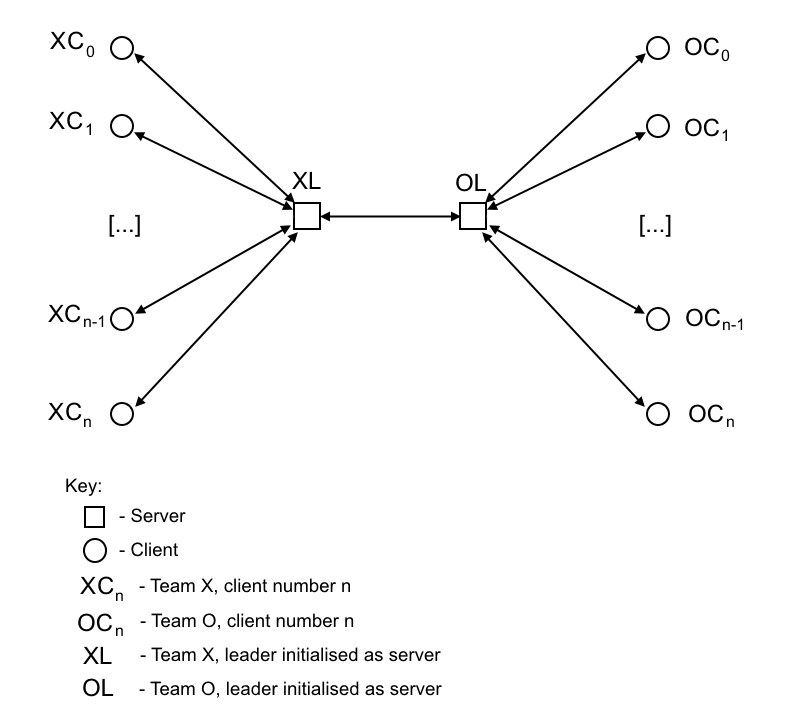
\includegraphics[width=\linewidth]{images/DAS-topology.png}
	\caption{Topology for Distributed Tic Tac Toe}
	\label{fig:topology1}
\end{figure}

The leaders communicate the vote of their team to the opposing leader so that they may pass that result on to the peers of that team, as pictured in figure 1.

By considering the fact that only the two leaders communicate about the votes between the two teams, then the system can easily break if one of the leaders creashes. 
In order to avoid that and provide a more robust system we chose to implemet the Bully Algorithm on each of the players so they will be able to detect a leader crash if they do not receive a vote reply from them in a certain period of time.
After that, they can easily call for an election on older processes than them and wait for a leader to be announced on a different period of time.
If no leader is announced on that period of time or there are no older processes, then that process can declare itself leader to the rest of the team and the opponent leader.

\section{Implementation}

The implementation follows the RMI distributed object model. A GameInt interface extends java.rmi.Remote and lists remote classes. 
A Game class implements GameInt and extends the UnicastRemoteObject. It is an analogy for what a player knows and does during a game. 
It provides an implementation for all the listed classes in the interface which include the functionality of requesting the player to make a play, 
setting the leader of the game, several methods to interact with the Role of the player and a main method that connects to other game instances. 
Currently, when running the game, the user passes it a local instance name and the name of another instance as arguments. Each instance then uses this information 
to do an RMI Registry lookup and get a reference to the other client. The Role interface allows the application to differentiate between Leader and Player classes which extend it. 
It utilises the State design pattern to allow players to seamlessly have their role changed – for example when the current leader disconnects. 
A Leader is responsible of collecting the votes from all of the members in their team in the turnStarts() method. This is done asynchronously using
a separate thread for each member – an instance of VoteThread. Each thread collects a vote from one assigned player then writes it into a corresponding position
in a shared AtomicIntegerArray that they have all been passed by the Leader. This ensures the main Leader thread can then read these values. 
Each Leader then informs all players in the game about the vote of his team. A Player instance represents a regular player that only must vote. 
Each regular player also has a mechanism to detect if a leader has not contacted them to choose a play for too long. If a time-out is triggered, 
a player calls for a new leader election. To avoid many simultaneous election calls, each regular player waits 5 minutes plus a randomised amount of time.
All plays are recorded on a GameState object instance that acts as a game board. After each turn it checks if the game is over and relays this message to the leaders
 which can then inform the members of their team.
 
 
% Bully Implementation
% All of the players keep track of their leader, the opponent leader and a priority list of their team.
% In this case, they can easily use the list to start election on the processes older than them.

\section{Evaluation}

\section{Related Work}
While other multiplayer distributed games already exist, they have not been
created with this project’s task in mind and therefore do not serve the same
purpose. They can be split into two categories – very unprofessional and too
professional. For example, hobby implementations exist that deal with
distributed problems in a bad fashion, promoting bad and incorrect programming 
practises. Similarly, a single-player-per-team distributed tic-tac-toe game in 
Java can be found online that does not comply with any design guidelines and 
puts all functionality in a single class and as such, cannot teach students good 
practice and has the potential of confusing the learner further about distributive 
programming \cite{MrWayFarOutYoutube15}.

Separately, very in-depth materials that provide state-of-the-art practices can 
be found \cite{DBLP:conf/nsdi/BharambePS06} but there is a high possibility that they might be incomprehensible 
to a beginner reader looking to tackle basic distributed concepts to begin with. 
Furthermore, none of the similar implementations residing on the Internet take advantage 
of the Java RMI API which must be considered a good starting point for distributed systems
learners for it to be taught as part of our degree and is a requirement for this
project. Instead, they use different sets of other technologies which can
further confuse their reader and introduce a steeper learning curve.

\section{Conclusions and Future Work}

% trigger a \newpage just before the given reference
% number - used to balance the columns on the last page
% adjust value as needed - may need to be readjusted if
% the document is modified later
%\IEEEtriggeratref{8}
% The "triggered" command can be changed if desired:
%\IEEEtriggercmd{\enlargethispage{-5in}}

% references section

% can use a bibliography generated by BibTeX as a .bbl file
% BibTeX documentation can be easily obtained at:
% http://mirror.ctan.org/biblio/bibtex/contrib/doc/
% The IEEEtran BibTeX style support page is at:
% http://www.michaelshell.org/tex/ieeetran/bibtex/
\bibliographystyle{IEEEtran}
\bibliography{references}
\end{document}
